% !TEX root = pfe-book3.tex
%!TEX TS-program = pdflatex
%!TEX encoding = UTF-8 Unicode


\cleardoublepage
%\mainmatter
\chapter{Radio}
\label{ch-06}

\section{Some History}

Just as Faraday had no idea that the discovery of electromagnetic induction would lead to the founding of electrical engineering, and Ernest Rutherford considered idle talk and rank ignorance the feasibility of extracting energy from the atomic nucleus, so Heinrich Hertz, after discovering electromagnetic waves and showing how they can he detected at distances of several metres, had no notion of radio communication and even denied its possibility. Three amusing facts, are they not? But we shall leave their discussion to the psychologists.


Therefore, restricting ourselves to a mere statement of this remarkable circumstance, we shall see how events developed after Hertz's early death in 1894.
Hertz's classical experiments, which we have described in such detail, attracted the attention of scientists all over the world. Professor N. G. Yegorov of the St. Petersburg University accurately repeated these experiments. The spark in the resonator was barely visible. It could be seen only in complete darkness and then only with a magnifying glass.

Alexander Stepanovich Popov (1859-1906), an unassuming lecturer in electrical engineering at the Kronstadt Military Academy, set to work in 1889, at the age of 30, to improve Hertz's experiments. The sparks that he obtained in his resonators were much fatter than those other investigators succeeded in producing.

In 1894, a fall issue of the English journal \emph{Electrician} published an article by the well-known English physicist Sir Oliver Joseph Lodge (1851-1940) in which he claimed that Hertz's resonator could be improved by using the Branley tube. The French scientist Edouard Branley (1844-1940) was engaged in research on the conductivity of metal filings. He found that such filings do not always offer the same resistance to electric current. Loosely packed metal filings in a tube have practically infinite resistance, but if the tube is placed in the vicinity of an operating Hertz resonator, the resistance drops drastically. The explanation is that the small filings cohere owing to the welding action of the tiny sparks produced between them by the electromagnetic wave. When lightly tapped or shaken, the resistance of the filings is restored.

This property of metal filings was made use of by Lodge. He wired a circuit consisting of the Branley tube (which came to be known as a \emph{coherer}), a battery and a sensitive galvanometer. The hand of the instrument was deflected at the instant electromagnetic waves passed by. Lodge succeeded in detecting radio waves at distances up to \SI{40}{\meter}.

This system was inconvenient, however, because the coherer immediately stopped operating. It was necessary to find a way to restore the cohering (welded) filings to their initial state, with the required device designed so that the shaking occurs automatically.

%\newpage

\begin{center}
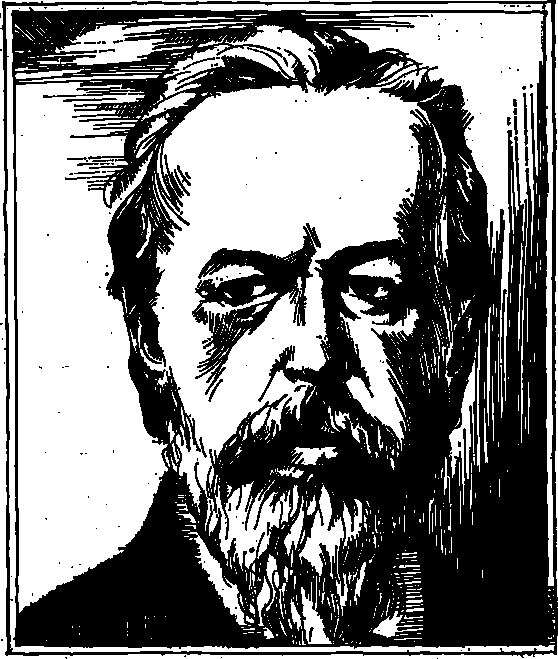
\includegraphics[width=0.8\textwidth]{figures/popov.pdf}
\end{center}
{\small \textsf{{Alexander Stepanovich Popov [1859-1906]}} -- \textsf{\footnotesize great Russian physicist and electrical engineer; invented the radio. Popov's scientific work was highly appraised by his contemporaries. In 1900 he won a Gold Medal at the World's Fair in Paris for his invention.}}


This problem was solved by Popov. He tried many kinds of coherers and finally decided to use one designed as follows (\figr{fig-6.1}). ``Two strips of thin sheet platinum, $AB$ and $CD$, are glued on the inside wall of a glass tube and extend over almost the whole length of the tube. One strip emerges at one end of the tube and the other strip at the other end. The strips are \SI{8}{\milli\meter} wide and are arranged with a space of about \SI{2}{\milli\meter} between them. The inner ends, $B$ and $C$, of the strips do not reach the corks that plug the tube so that filings jammed between the cork and the tube cannot form conducting chains that cannot be broken up when the tube is shaken. This happened in some of the earlier models. The length of the whole tube is from 6 to \SI{8}{\centi\meter} and its diameter is about \SI{1}{\centi\meter}. In operation the tube is arranged horizontally so that the strips are at the bottom and are covered by metal filings. Best operation is achieved when the metal filings fill not over one-half of the space in the tube.''


\begin{figure}[!ht]
\centering
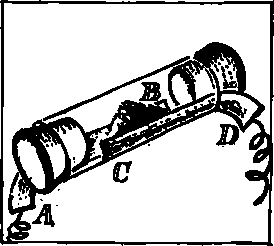
\includegraphics[width=0.4\textwidth]{figures/fig-06-01.pdf}
\caption{Popov's coherer.}
\label{fig-6.1}
\end{figure}

Popov's coherer, just described in his own words, is shown in \figr{fig-6.1}. He used iron or steel powder in it. The main problem, however, was not to improve the
coherer, but to invent a method of restoring its initial state after detecting an electromagnetic wave. In Popov's first receiver, whose wiring diagram is shown in \figr{fig-6.2}, this job was performed by an ordinary electric bell. The striker of the bell replaced the galvanometer hand and its hammer struck the glass tube when the striker returned to its initial position.

\begin{figure}[!ht]
\centering

\includegraphics[width=\textwidth]{figures/fig-06-02.pdf}
\caption{Wiring diagram for Popov's receiver.}
\label{fig-6.2}
\end{figure}

What a simple solution of a puzzling problem! And really simple. Do you realize, dear reader, that this elementary arrangement, which neither Hertz nor Lodge hit upon, was the first application of what engineers now call a relay circuit? The negligible energy of radio waves is not directly detected, but is used to control a current circuit.

In the spring of 1895, Popov set up his apparatus outside, in an orchard. He began to move the receiver farther and farther away from the oscillator. At \SI{50}{\meter} the bell responded to the spark of the oscillator; at \SI{60}{\meter} the apparatus still worked, but at \SI{80}{\meter} the bell refused to ring. Then Popov took a coil of copper wire, threw one end up into a tree and connected the other end to the coherer. The bell rang. This is how the first antenna was devised.

In the USSR, the 7th of May is celebrated each year as Radio Day. On this day in 1895 Popov read a paper with the unassuming name ``On the Relationship of Metal Powders to Electric Oscillations'' at the regular session of the Russian Physico-Chemical Society. Many of those present had watched a demonstration, several years previously, of Hertz's experiments in which the tiny sparks could be seen only through a magnifying glass. But, when they heard the brisk clangour of Popov's receiver, they realized that they were witnessing the birth of the wireless telegraph, that a new and more efficient method of transmitting signals over long distances had been invented.

On March, 12, 1896, Popov transmitted the world's first radiogram. By pressing a key for short and long intervals, the words ``Heinrich Hertz'' were transmitted over a distance of \SI{250}{\meter} from one building to another and were recorded on telegraph tape.

By 1899, the range of radio communication between the training ships of a mine-layer detachment had already reached \SI{11}{\kilo\meter}. The practical importance of the wireless telegraph was no longer doubted even by the most skeptical officials.

The Italian electrical engineer and inventor Guglielmo Marconi (1874-1937) began his experiments somewhat later than Popov. Marconi carefully followed all the advances in the fields of electrical engineering and the study of electromagnetic waves. He skilfully employed them to improve the quality of radio reception and transmission. His especial contribution was more in the line of organization and management rather than the strictly technical aspect. This is no small matter, however, and Marconi's fame is well deserved. We should not forget that the priority in the discovery of the radio, based on the paper read on May 7, 1895, belongs to the unpretentious Russian scientist Popov who always refused to put his knowledge and research at the disposal of any country except his native land.

Marconi did not mention Popov in his articles and lectures. But not everyone knows that in 1901 he offered Prof. A. S. Popov a position in the commercial company that Marconi had founded and was the president of the range of.

The range of radio reception grew at a rapid rate. In 1899, Marconi established radio communications between France and England, and in 1901 a radio signal was sent from Europe to America.

What technical innovations facilitated these successes and made radio broadcasting feasible?

Beginning with 1899, radio engineering no longer based reception on the coherer. Instead of detecting radio waves by the drop in the resistance of a circuit due to the effect of an electromagnetic wave, an entirely different technique can be made use of. A rectified pulsating electromagnetic wave can be detected by the clicks heard in an ordinary telephone receiver.

This began a search for rectifiers. The extensively used contact detector, applied right up to the twenties of our century, consisted of a crystal with one-way conduction. Such crystals had been known since 1874. They include metal sulphides, copper pyrites and hundreds of different minerals. People of my age remember such radio sets and the irritating procedure of searching for ``good contact'' with a whisker (contact spring). Such contact was achieved when the point of the whisker had found a ``suitable'' spot on the crystal (\figr{fig-6.3}). By that time many broadcasting stations were in operation so that the set had to be tuned to the required wave. This was done with a multicontact switch for a small number of stations, or by steplessly varying the capacitance of the capacitor, which is also employed in up-to-date apparatus.

\begin{figure}[!ht]
\centering
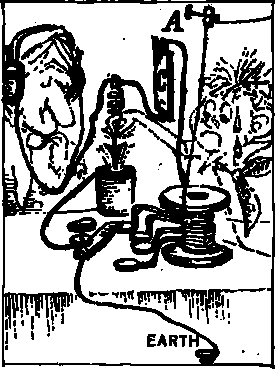
\includegraphics[width=0.4\textwidth]{figures/fig-06-03.pdf}
\caption{Finding the whisker contact on radio.}
\label{fig-6.3}
\end{figure}

It was extremely difficult, or even impossible in some cases, to operate at high power with the spark-gap broadcasting stations because the spark-gap device became overheated. Such stations were soon replaced by one operating on the principle of an oscillating electric arc or a high-frequency alternator. After this the power ratings reached hundreds of kilowatts.

The real revolution in radio communications, enabling speech and music to be transmitted instead of only telegraph code, came with the development of the vacuum tube.

In October 1904, the English electrical engineer Sir John Ambrose Fleming (1849-1945) showed that high-frequency current could be rectified by a vacuum tube consisting of a filament heated by the current and surrounded by a metal cylinder. Its diagram is illustrated in \figr{fig-6.4}. Fleming realized the value of the vacuum-tube diode for converting electric oscillations into sound (he called this device a ``valve'' because it opened and shut the gate to the flow of electricity), but he could not achieve wide application of his detector.

\begin{figure}[!ht]
\centering
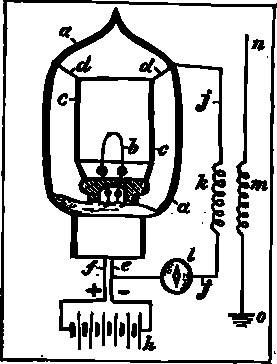
\includegraphics[width=0.4\textwidth]{figures/fig-06-04.pdf}
\caption{A vacuum-tube structure and operational setup.}
\label{fig-6.4}
\end{figure}


The fame of inventing the electron lamp was won by the American scientist Lee de Forest (1873-1961). In 1906, he converted the two-electrode tube (diode) into a triode by adding a third element. The tube was called an \emph{audion} (from the Latin word \emph{audire}, meaning \emph{I hear}. De Forest's vacuum tube radio set received signals on the grid (third element) in the lamp, rectified them and enabled them to be heard as telegraph code in headphones.

The feasibility of using the electron tube as an amplifier was evident to the American scientist. But only after seven years had passed, in 1913, a triode was first applied in a generator circuit by the German radio engineer Alexander Meissner (1883-1958).

Attempts to transmit speech, i.e. the modulation of an electromagnetic wave, had been made before the electron tube was used as a generator. But the difficulties were very great: the band of frequency modulation could not be made wide enough. Speech could be transmitted with some little success, but not music. Only in the twenties did radio transmitters and receivers, operating with electron tubes, demonstrate the truly inexhaustible capabilities of radio communications for transmitting the whole range of audio frequencies.


The next revolutionary breakthrough occurred not long ago, when semiconductor elements superseded electron tubes in radio circuits. This established a new branch of applied physics dealing with the huge complex of problems concerning the input, transmission and storage of information.

\section{Vacuum-Tube Triode and Transistor}

Vacuum-tube triodes incited an upheaval in radio engineering. But technology ages faster than people do. Today, the electronic tube has become a pensioner or, as they say in the USA, a senior citizen. Not so many years ago you could hear impatient prospective customers in shops selling TV sets demanding transistorized models, i.e. sets in which semiconductors have replaced electronic tubes.

But age demands respect. Moreover, the principles underlying the two fundamental applications of tubes and transistors, namely, the amplification and generation of waves of a definite frequency, can be more simply described by using the electronic tube as an example.


\begin{figure}[!ht]
\centering
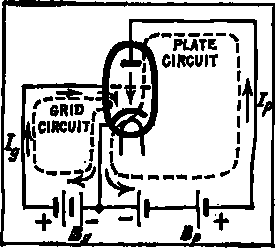
\includegraphics[width=0.5\textwidth]{figures/fig-06-05.pdf}
\caption{Schematic showing how the grid enables plate current to be controlled.}
\label{fig-6.5}
\end{figure}

We shall therefore cover its operation in more detail than that of the transistor.
Besides the plate (anode) and heated filament (cathode), the bulb of a three-electrode tube has a sealed-in third electrode, called the grid. The electrons freely pass through the grid. Its openings are as much larger than the electron as the earth is larger than a dust speck. \figr{fig-6.5} illustrates how the grid enables the plate current to be controlled. It is evident that a negative voltage impressed on the grid reduces the plate current and a positive voltage increases this current.


\begin{figure}[!ht]
\centering
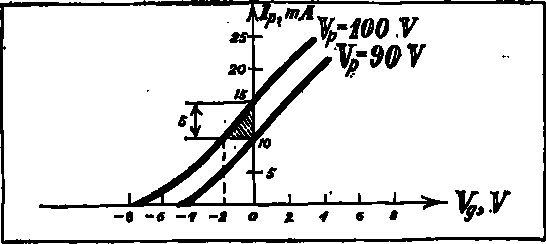
\includegraphics[width=\textwidth]{figures/fig-06-06.pdf}
\caption{Tube characteristic curve.}
\label{fig-6.6}
\end{figure}


Let us conduct a simple experiment. First we apply 100 volts across the cathode and anode (filament and plate). Then we begin to vary the grid voltage as shown, for instance, in \figr{fig-6.6} in a range from minus eight volts to plus five. Using an ammeter, we measure the current in the plate circuit. From this data we can plot the upper curve shown in \figr{fig-6.6}. This is called the \emph{tube characteristic}. Next we repeat the experiment with a plate voltage of 90 volts. We obtain a similar curve (lower curve in \figr{fig-6.6}).

Take note of the following outstanding feature. As is obvious from the hatched triangle, we can increase the plate current by 5 milliamperes in two different ways: either by increasing the plate voltage by 10 volts or by increasing the grid voltage by 2 volts. The introduction of the grid makes an amplifier out of the vacuum-tube triode. The amplification factor in our example equals 5 (ten divided by two). In other words, the effect of the grid voltage on the plate current is five times that of the plate voltage.

Now, we shall discuss how a triode enables us to generate waves of a definite length.

\begin{figure}[!ht]
\centering
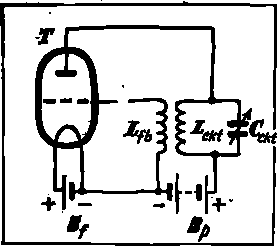
\includegraphics[width=0.4\textwidth]{figures/fig-06-07.pdf}
\caption{Working of a triode.}
\label{fig-6.7}
\end{figure}

This is illustrated by the extremely simplified circuit diagram given in \figr{fig-6.7}. When the plate voltage is applied (switched on), capacitor $C_{\textrm{ckt}}$ of the oscillatory circuit is charged through the tube. The lower plate is positively charged. The capacitor is immediately discharged through the inductor $L_{\textrm{ckt}}$. This produces free (natural) oscillations that would be damped if there were no continuous energy input from the tube. How can we ensure that this energy is supplied at the proper times so that the oscillatory circuit builds up in the same way as the amplitude of a swing when you push it at the right times? This requires what is called \emph{feedback}. The current of the oscillatory circuit induces an emf in coil $L_{\textrm{fb}}$, of the same frequency as that of free oscillations. Thus the grid produces a pulsating current in the plate circuit; this current builds up the circuit with its natural frequency.



The two ingenious principles described above are the basis on which radio engineering and allied fields have been established. The electronic tube has become obsolete, making way for the transistor, but the idea of amplifying and generating electromagnetic oscillations has remained the same.

As in a vacuum-tube triode, low power in the input circuit of a transistor can control high power in the output circuit. There is a difference in the way control is accomplished. The plate current of a tube, as we have seen above, depends upon the grid voltage. The current of a collector in a transistor depends on the emitter current.

But we have not described a transistor yet. It has three electrodes. The emitter corresponds to the cathode, the collector to the plate (anode) and the base to the grid. The lead from the emitter is the input and that from the collector is the output.

\begin{figure}[!ht]
\centering
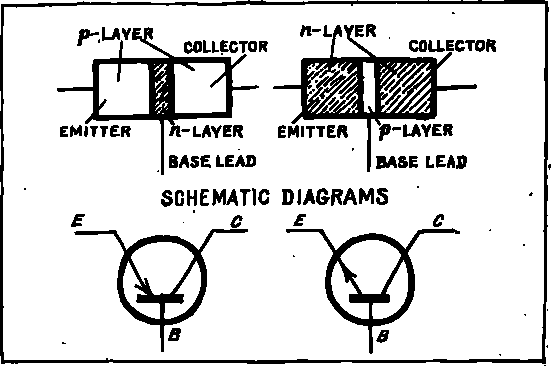
\includegraphics[width=\textwidth]{figures/fig-06-08.pdf}
\caption{The \emph{n-p-n} and \emph{p-n-p} transistors..}
\label{fig-6.8}
\end{figure}

As shown in \figr{fig-6.8}, the transistor consists of two \emph{p-n} junctions. At the left is \emph{p-n-p} transistor with the \emph{n}-layer in the middle between two \emph{p}-layers. We can also have a \emph{p}-layer in the middle, in which case we have an \emph{n-p-n} transistor (at the right).

We always bias the emitter positively so that it can produce a large number of majority carriers of charges. When the low-resistance emitter circuit changes the current in the high-resistance collector circuit, we obtain amplification.
The ways in which transistors are connected into circuits and employed as amplifiers and generators are similar, in the main, to the principles of the vacuum-tube triode. But we shall not discuss this extremely vital branch of up-to-date physics here.


\section{Radio Transmission}

The kinds of radio transmission can be classified on the basis of the power rating of the broadcasting station. Large stations transmit signals at powers ranging up to a megawatt. A miniature transmitter of the walkie-talkie type, employed by a traffic cop to notify his colleague that a Lada car with the license number 31416P has just jumped a stop light and is to be held up, radiates about one milliwatt. Even less power is sufficient for some purposes.

There are essential differences in the layout and design of stations operating with waves over several metres long and transmitters radiating ultrashort waves with a length of dozens of centimetres or even only fractions of a centimetre. Within each of the wavelength and power ranges, the engineer designing the station can apply any of a huge number of circuits and layouts that may be dictated by the locality, specific aims, economic considerations or, simply, engineering intuition.

The basic unit of a radio transmitter is the radio wave generator, or oscillator. What kind will you employ? You have at least five choices. You can use a vacuum-tube oscillator. Its range is exceptionally wide. Power ratings may vary from fractions of a watt to hundreds of kilowatts, and frequencies from dozens of kilohertzes to several gigahertzes. But if your power requirement is small, of the order of tenths of a watt, only a transistor oscillator will suit you. On the contrary, you will have to reject transistors for the time being (probably not for long) if your power requirement exceeds several hundred watts. If, however, the power rating is such that both types of oscillators can be efficiently applied, the designer will evidently prefer the transistor version. Such an engineering solution is doubtlessly more elegant.

A transistorized transmitter occupies considerably less space and, if necessary, can much more easily be designed as a portable model than a transmitter with a vacuum-tube oscillator.

Magnetron and klystron oscillators have more specialized application. The former can be extremely useful in sending pulses of several megawatts into space. The frequency band for which magnetron oscillators can be used is much narrower: it lies approximately between 300 megahertzes and 300 gigahertzes.

Klystron oscillators are used for the same range of ultrashort waves. But they find application only in low power installations: not exceeding several watts in the centimetre and several milliwatts in the millimetre bands.

The last two types of oscillator, as well as the fifth type, the quantum oscillator, are highly specific and require a special discussion. As to transistor and vacuum-tube transmitters, they resemble each other. There is a clear-cut engineering rule enabling one to replace a vacuum tube with an equivalent transistor.

The choice of the generator of electromagnetic oscillations is by far not all that is required for designing a transmitter. You must decide how to amplify the power produced by the primary (or, as they say, master) oscillator. You must also select a method for modulating the carrier wave by the audio frequencies. There are also many ways for transmitting power to the antenna field. The arrangement of the antenna field itself provides abundant opportunity for exercising engineering ingenuity.
\begin{figure}[!ht]
\centering
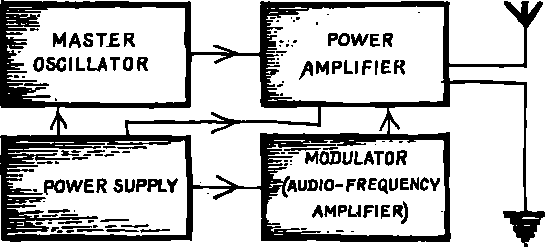
\includegraphics[width=\textwidth]{figures/fig-06-09.pdf}
\caption{A block diagram of a radio broadcasting station.}
\label{fig-6.9}
\end{figure}

Radio engineers frequently resort to so-called \emph{block diagrams}. Such a diagram consists of several rectangles with captions. The contents of each rectangle is cleared up as required. A block diagram of a radio broadcasting station is illustrated in \figr{fig-6.9}. The master oscillator generates continuous, almost harmonic, oscillations of the same frequency and wavelength to which you tune
your radio receiver if you wish to listen to the given station. The second unit is the power amplifier. Its name speaks for itself and we shall not describe its design. The task of the unit called the modulator is to convert sound vibrations into electric oscillations and superimpose them on the carrier wave of the broadcasting station.

Modulation can be accomplished in various ways. The simplest kind to explain is frequency modulation. In many designs the microphone is a capacitor whose capacitance is varied by the sound pressure because the capacitance depends upon the distance between the plates. Imagine now that such a capacitor is connected into the oscillatory circuit which generates the wave. Then the frequency of the wave varies with the sound pressure.

Since we have ``invaded'' the oscillatory circuit with our microphone, a band of frequencies is transmitted into space rather than a strictly definite frequency. It is sufficiently evident that ideally this spreading should include the whole audio interval of frequencies which, as we know, equals about 20 kHz.

If the station is broadcasting on long waves, corresponding to a frequency of the order of 100 kHz, the passband is about one-fifth of the carrier frequency. It is clear that long waves cannot provide for a large number of non-overlapping broadcasting stations. Short waves are an entirely different matter. For a frequency of 20 MHz, the band width is only a fraction of one per cent of the carrier frequency.

There is probably not a single home in the USSR that has no plug socket for listening to the radio. You receive these broadcasts from the so-called rebroadcasting network. It is also called wire broadcasting.

The first single-program rebroadcasting network was established in Moscow in 1925. The broadcast was transmitted simultaneously through 50 loudspeakers.


Single-program rebroadcasting is carried out on audio frequencies. From the broadcasting station, the program is transmitted by wire to the central amplifying station. From the central station it is transmitted, again by wire, to the control points, where it is again amplified and transmitted along the trunk feeder mains to the transformer substations. From each substation the wires branch off to substations of the next lower rank. Depending upon the size of the city or region, the number of steps in the network and, consequently, the number of times the voltage is stepped down, may vary. In the subscriber's lines the voltage is equal to 30 V.

Since 1962, three-wire rebroadcasting is being installed in the cities of the USSR. The transmission of two additional programs is accomplished along independent networks by amplitude modulation on carrier frequencies of 78 and 120 kHz. These two broadcasts are demodulated (i.e. the sound is separated out and the high frequency is filtered out) in the home by turning the knob of your Mayak wire-broadcasting plug-in receiver or some other model.

Thus, in three-program rebroadcasting, a single wire carries three programs simultaneously: the main program is on audio frequencies and two are non-demodulated. Therefore, the broadcasts do not interfere with one another. A simple idea, but what excellent results! Economy, reliability and high fidelity of the broadcasts are factors that indicate that wire broadcasting has a great future, including the installation of wire networks for television.

\section{Radio Reception}
Radio receiving sets are available in innumerable designs. The field of radio electronics is being developed at an exceptionally rapid rate, so that radio sets soon become obsolete and new items, better than the previous models, are available each year in the shops.

What do we mean by ``better'' with respect to receivers? Each and every reader knows the answer even if he does not understand the physics involved. A good receiving set must separate out of the chaos of radio waves that reach the antenna only those signals that are required. This property is called \emph{selectivity}. A radio set must also be as sensitive as possible, i.e. it should he able to receive even the weakest signals. Finally, it must have high fidelity, i.e. it must reproduce the music and speech broadcasted from the tuned-in station without any distortion whatsoever.

Thus, sensitivity, selectivity and fidelity. We could, perhaps, add one more requirement: the set should operate well on all wave bands.

\begin{figure}[!ht]
\centering
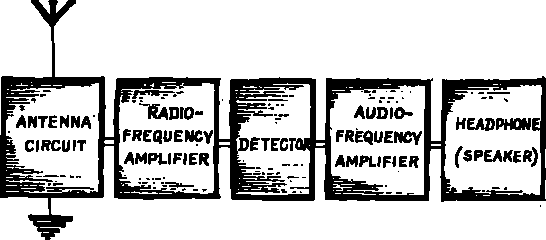
\includegraphics[width=\textwidth]{figures/fig-06-10.pdf}
\caption{A block diagram of a radio receiver.}
\label{fig-6.10}
\end{figure}

The block diagram of a receiver with straight amplification is sufficiently clear (\figr{fig-6.10}). It is necessary, first of all, to separate out the required wavelength and to amplify the radio-frequency oscillations produced in the antenna by the wave of the broadcasting station. Next, it is necessary to accomplish rectification, or demodulation, which is the name of the process of ``discarding'' the carrier frequency and sifting out the information carried by the sound from the electric current. Finally, it is necessary to provide one more amplifier, but for audio frequencies. The concluding stage is to convert these electric oscillations into sound. This is done by means of a dynamic loudspeaker or by headphones. The latter are used by considerate people who do not wish to be a nuisance to their neighbours.


\begin{figure}[!ht]
\centering
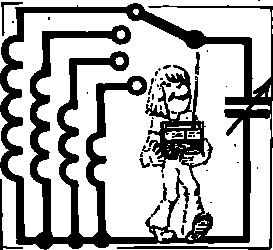
\includegraphics[width=0.4\textwidth]{figures/fig-06-11.pdf}
\caption{Schematic block diagram of antenna linked to inductive oscillatory circuits for tuning.}
\label{fig-6.11}
\end{figure}


The antenna of the receiving set is usually inductively linked to the oscillatory circuits of several frequency bands. When we turn the band switch knob, we perform the operation shown schematically in \figr{fig-6.11}. Within the limits of each band we usually tune the set by varying the capacitance of the oscillatory circuit capacitor. The capacity of the radio set to select the frequency in the optimal way is determined by the resonance curve of the oscillatory circuit.

I am looking at the specifications in the instruction book of an automobile radio set. Its selectivity is within 9 kHz of resonance for the long- and medium-wave frequency bands. This, of course, is not the limit that can be reached.

The sensitivity of a radio receiver is characterized by the minimum emf in its antenna that enables us to hear the broadcast with sufficient clarity (I cannot say that this definition is very exact). In the automobile radio set the sensitivity for long waves is better than \SI{175}{\micro\volt} and for ultrashort waves, better than \SI{5}{\micro\volt}.

The sensitivity depends upon the amplification factor and on set noise. The amplification factors of radio sets vary from \num{d5} to \num{d8}. This means that the broadcasting station I want to listen to must produce an induced emf of at least \SI{d-8}{\micro\volt} in the antenna of the receiver.

\section{Radio-Wave Propagation}

The simplest case is the propagation of radio waves in free space. At a relatively short distance away the radio transmitter can be regarded as a point. If so, then the radio wave front can be assumed spherical. If we imagine several spheres concentrically surrounding the transmitter, it will be clear that, in the absence of absorption, the energy passing through the spheres remains constant. As we know, the surface of a sphere is proportional to the square of the radius. Hence, the wave intensity, i.e. the amount of energy transmitted by the wave in unit time through unit area perpendicular to the direction of wave propagation, decreases as we move away from the source in inverse proportion to the square of the distance.

This important rule is applicable, of course, if no special measures have been taken to obtain a narrow directed beam of radio waves.

Various techniques exist for producing directed radio beams. One way is to use the proper beam, or antenna, array. The antennas should be arranged so that the waves they transmit are sent in the required direction, ``hump to hump''. Reflectors of various shapes are also employed for this purpose.


Radio waves travelling in space may deviate from the straight-line direction of propagation by being reflected, dispersed or refracted if they meet with an obstacle commensurate with the wavelength.

Of greatest interest is the behaviour of waves travelling near the surface of the earth. Each case may prove to be entirely unique, depending upon the wavelength.
Of cardinal importance are the electrical properties of the earth's surface and of the atmosphere. If the surface can conduct a current, it does not ``release'' the radio waves. Electric lines of force of an electromagnetic field enter a metal (or, for that matter, any conductor) at a right angle.

Now just imagine that the radio transmission is near the surface of the sea. Sea water contains dissolved salts and is therefore an electrolyte. Sea water is an excellent current conductor. Consequently, it ``holds'' the radio waves, making them travel along the surface of the sea.

Plains and timbered areas are also good conductors for currents of not especially high frequency. In other words, plains and forests behave like metals with respect to long waves.

For these reasons, long waves are contained by the whole surface of the earth and are capable of circumventing the globe. Incidentally, the velocity of radio waves can be measured in this way. Radio engineers know that it takes a radio wave 0.13 second to go around the earth. How about mountains? As far as long waves are concerned, mountains are not so high, and a wave a kilometre long can go around a mountain with more or less ease.

The feasibility of long-range reception of short waves is based on the presence of the ionosphere. The sun's rays are capable of breaking up the molecules of air in the higher regions of the atmosphere. The molecules are converted into ions and form several charged layers at altitudes from 100 to 300 km. Thus, the space through which waves of short length travel is a layer of dielectric sandwiched between two conducting surfaces.

Since plains and forest lands are poor conductors for short waves, they are incapable of holding them. Short waves depart on their journey into free space but encounter the ionosphere which reflects them like the surface of a metal.

The ionosphere is nonuniformly ionized and this varies from day to night. Therefore, short radio waves may travel along various paths. They may reach your radio set after being reflected time after time by the ionosphere and the earth. The actual fate of any short wave depends upon the angle it makes with the ionosphere layer. If this angle is close to a right angle, no reflection occurs and the wave goes through and off into outer space. More frequently, however, total internal reflection takes place and the wave returns to the earth.

The ionosphere is transparent to ultrashort waves. Radio reception of such waves is therefore possible only along a line of sight (with the receiver antenna within sight of the transmitting antenna) or with the aid of communications satellites. If we direct our wave at the satellite, we can pick up the signals reflected from it at enormous distances.

Satellites ushered in a new era in radio communications techniques by making radio and TV reception feasible on ultrashort waves.

Transmission by centimetre, millimetre and submillimetre waves presents extremely interesting opportunities. Waves of this length can be absorbed by the atmosphere. It was found, however, that there are ``windows'' and, if the wavelength is properly selected, we can make use of waves that are already within the optical band. The advantages of such waves are well known: in a narrow wave band we can ``fit in'' a huge number of non-overlapping broadcasts.

\section{Radar}
The principles of radar (\textbf{ra}dio \textbf{d}etecting \textbf{a}nd \textbf{r}anging) are sufficiently simple. We transmit a signal, it is reflected by the object that interests us and returns to our receiver. If the object is 150 m away, the signal returns in 1 microsecond, if the distance is 150 km, it returns in 1 millisecond. The direction in which the signal returns is along a line from the point where the airplane, rocket or automobile was at the instant it met the radio beam.

Naturally, the radio wave must be a pencil beam; the angle of the beam, within which the greater part of its power is concentrated, should be of the order of one degree of arc.

The principle is really not at all complicated, but the apparatus required is far from simple. To begin with, exceptionally high requirements are made to the oscillator. Vacuum-tube oscillators are used for the metre and decimetre bands (longer waves are obviously inapplicable), and klystrons and magnetrons, for the centimetre band.

The pulsed system of operation is evidently the most natural one. Very short pulses are periodically transmitted into space. The duration, or length (of time), of the pulse ranges from 0.1 to 10 microseconds in up-to-date radar transmitters. The frequency of the pulses must be selected so that the echo signal has time to return and be received in the pause before the next pulse is sent.

The maximum range at which an airplane or rocket can be detected is limited only by the condition that the object must be on a line of sight from the radar set. The reader knows, without doubt, that up-to-date radar installations are capable of picking up signals reflected from any planet of our solar system. The waves they use must, of course, pass unimpeded through the ionosphere. Fortunately, shortening the wavelength also has a direct effect on the range of radar operation because this range is proportional to the frequency of radiation and not only to the energy of the transmitted pulse.

Traces of the transmitted and received pulses are visible on the screen of an oscilloscope (cathode-ray tube). If the airplane is flying toward the observer, the trace of the echo signal moves toward the trace of the transmitted pulse.

Radar installations do not necessarily have to operate with a pulsed system. Assume that the airplane is flying toward the transmitter antenna with the velocity $v$. The radio beam is being continuously reflected from the airplane. Due to the Doppler effect, the frequency of the received waves is related to that of the transmitted waves by the equation
\begin{equation*}%
v_{r} = v_{tr} \left( 1 + \frac{2v}{c} \right)
\end{equation*}
Frequency values are determined with great precision by radio engineering methods. By tuning into resonance, we determine the value of $\nu$ and from it we calculate the airplane's velocity $v$. If, for instance, the frequency of the transmitted signal equals \SI{d9}{\hertz} and the airplane or rocket is approaching the radar antenna at a velocity of \SI{1000}{\kilo\meter\per\hour}, the received frequency exceeds the transmitted frequency by \SI{1850}{\hertz}.

The reflection of a radar beam from an airplane, rocket, steamship or automobile is not the same as from a reflector. The wavelength is commensurate with or substantially smaller than the size of the reflecting object which, moreover, is of a complex shape. As the rays are reflected by various points of the object, they (the rays) interfere with one another and are scattered to the sides. Owing to these two phenomena, the effective reflecting surface of the object differs considerably from its true surface. Calculations here are extremely complicated and only the skill and experience of the radar operator enable him to determine what kind of object is encountered by the radar beam.

You have, of course, seen radar antennas: large spherical reflectors of wire lattice structure, always in motion, surveying space. A great many different kinds of motion can be imparted to the radar reflector. For example, the beam can be moved so that it scans space in lines or circles. With this mode of operation, the path of flight of the airplane can be followed besides determining its range.
This technique is used to home aircraft into an airport under conditions of a total lack of visibility. This job may be done either by a person or even by an automatic device.

A radar set can be ``deceived''. In the first place, the object can be covered by a material that absorbs radio waves. Coal dust or rubber can be used for this purpose. Moreover, to reduce the reflection factor, the coating may be corrugated so that the major part of the radiation is disorderly scattered in all directions. If packages of aluminium foil strips or metallized fibres are thrown overboard from the airplane, the radar set is completely disoriented. This trick was first used by the English flying forces during World War II. A third way is to fill space with false radio signals.

Radar is an interesting field of engineering and has found extensive applications for peaceful purposes. It is impossible to conceive of defense today without the use of radar.

A competitor of radar is the laser (\textbf{l}ight \textbf{a}mplification by \textbf{s}timulated \textbf{e}mission of \textbf{r}adiation). The principles of location and ranging with a laser in no way differ from those described above.

Communication between spacecraft and the earth is based on the principles of radar. Radio telescopes are located so that they keep the spacecraft in view. The antennas of these telescopes are of huge size, some hundreds of metres in diameter. Such large antennas are required so that they can transmit powerful signals and pick up extremely weak signals from a radio transmitter. Of vital importance, naturally, is a narrow radio beam. If the antenna operates with a frequency of 2.2 thousand million oscillations per second (the wavelength being about 1 cm), the beam diverges only to a diameter of 1000 km over the distance to the moon. True, when the beam reaches Mars (300 million km away), its diameter is already equal to 700 000 km.

\section{Television}
Since 99 out of 100 readers daily spend an hour or two watching some TV program, it is only fair to say a few words about this wonderful invention. We shall discuss only the principles involved in television broadcasting and reception.

The idea of sending pictures over some distance consists in the following. The picture to be transmitted is divided into small squares. A physiologist can tell us how small the square must be for the eye not to be able to distinguish variations of brightness within it (the square). The luminous energy of each portion of the picture can be converted by the photoelectric effect into an electric signal. Next a way was devised for reading these signals. This is, of course, done in a strictly definite sequence as in reading a book. The electric signals modulate the electromagnetic carrier wave in exactly the same manner as in radio transmission. What happens further on is also identical to radio communications. The modulated oscillations are amplified and detected. The TV receiver reconverts the electric pulses into a visible image.

The televisor tube in the transmitter is called an image iconoscope, superorthicon or a vidicon. By means of a lens in the TV camera, the image is focussed on a photo-cathode. The most extensively used are cesium-oxide or cesium-antimony cathodes. The photocathode is mounted in an evacuated tube together with the target screen.

It is possible, in principle, to transmit an image by successively projecting the luminous flux from each element of the image. In this case, the photocurrent should flow only during the short time each element is being transmitted. Such operations would be inconvenient, however, and the camera tube contains a large number of photocells, rather than a single one, this number equalling the number of elements into which the image being transmitted is divided. This receiving screen is called the target and is of mosaic design.

The mosaic target is a thin plate of mica with a large number of grains of silver, insulated from one another and coated by cesium oxide, applied on one side. Each grain is a photocell. The other side of the mica plate is coated by a metallic film. A small capacitor is formed between each grain of the mosaic and the metal, and is charged by electrons emitted from the photocathode. It is evident that the charge of each small capacitor is proportional to the brightness of the corresponding spot on the image being transmitted.

Thus, a latent electric image of the object is produced in the metallic plate. How do we take it from the plate? By means of an electron beam which is made to scan the plate in the same way as the eye passes along the lines of print on the page of a book. The electron beam plays the role of a key switch which, for an instant, closes the electric circuit through a microcapacitor. At the instant the circuit is closed, the current is uniquely related to the brightness of the image.

Each signal can and should be amplified many times by the ordinary means applied in radio engineering. In transmitting the image, the eye should not be able to distinguish the fact that the electron beam is successively scanning the various spots of the luminous screen. A complete image, obtained on the screen of the kinescope in the TV receiver, during one cycle of electron beam motion, is called a frame. The frames must change at a frequency sufficiently high so that persistence of vision eliminates flickering of the picture being watched. 

What no-flickering frame frequency should be chosen? It must be a number related to the current frequency in the mains. The fact is that the pulsating voltage applied to the grid of the cathode-ray tube produces dark and bright lines on the screen. These lines are stationary and imperceptible only if the frequency with which the frames change is equal to or a multiple of the power mains frequency. Continuous motion is seen when the frames change with a frequency of at least \SI{20}{\hertz}; in television a frequency of \SI{25}{\hertz} is taken but a small flickering is still noticeable. It is undesirable to change the frames with a frequency of \SI{50}{\hertz} and therefore TV designers resorted to what is called \emph{interlacing} in the scanning process. The frequency is left at \SI{25}{\hertz}, but the electron beam (also called the \emph{exploring spot}) first scans the odd numbered lines and then the even numbered lines. Thus, the frequency with which the semi-frames change equals \SI{50}{\hertz} and any flickering in the brightness of the image becomes unnoticeable.

The frequency with which the frames change and the line-by-line scanning should be strictly synchronized. The technical details of this synchronization are beyond the scope of our book. Consequently, we shall not explain why the number of lines must be odd and consist of several whole factors. In the USSR the frame is divided into 625 lines, i.e, $5^{4}$. Since 25 frames are changed per second, lines are scanned with a frequency of \SI{15625}{\hertz}. From this condition follows the width of the band of TV signal frequencies.

The lowest frequency of \SI{50}{\hertz} is the semiframe frequency. The highest frequency is determined by the time required to transmit a single element.

Simple calculations, which we shall not carry out here, indicate that it is necessary to take \SI{6.5}{\mega\hertz} as the higher frequency. It follows that the carrier frequency must be at least 40 or \SI{50}{\mega\hertz}, because the frequency of the carrier wave must be at least 6 to 7 times the bandwidth of the transmitted frequencies. Now we understand why only ultrashort waves can be used in television transmission and why the range is limited to the line of sight from the transmitting antenna.

This, however, is a slip; I should have written: was limited. A breakthrough, enabling TV reception to be carried out at any distance, is the use of communications satellites. The USSR first employed satellites for this purpose. Today the whole of the Soviet Union is covered by communications accomplished by making use of a number of satellites.

Without going into the design of powerful TV stations, we shall only cite some interesting figures that characterize the huge possibilities possessed by up-to-date radio engineering in the amplification of signals. Before amplification, an ordinary video signal has a power up to \SI{d-3}{\watt}; the power amplifier increases this power by a million times. This pulse of \SI{d3}{\watt} is fed to a parabolic antenna about \SI{30}{\meter} in diameter. This antenna produces a narrow directed beam which is reflected by the satellite. After the electromagnetic wave has travelled about 35 000 km to the satellite, its power equals only \SI{d-11}{\watt}.

The amplifier mounted on the repeater satellite increases the power of this exceptionally weak signal to about \SI{10}{\watt}. When this signal, reflected from the satellite, returns to the earth, its power is \SI{d-17}{\watt}. Amplification returns the power of this video signal to its initial \SI{d-3}{\watt}.

I think that ten years ago not even the most optimistic engineer would have believed these figures.

\section{Microelectronic Circuits}
It is impossible to end this chapter devoted to radio engineering without at least a few words about the new revolution that we are witnessing in this field.
We have in mind the fantastic miniaturization of all electronic devices and apparatus. This became feasible in going over from apparatus built up of separate elements, such as resistors, transistors, etc., connected together by wiring, to electric circuits ``drawn'' by special techniques on a piece of silicon several millimetres in size.

This new technology (at least one of its versions) consists in using various kinds of masks and a series of chemical compounds enabling \emph{p}-type and \emph{n}-type impurities to be introduced at the required places of a crystal of silicon or germanium. Ion-beam treatment is used for this purpose.

An electric circuit consisting of tens of thousands of elements (!) is arranged on an area with linear dimensions of about two millimetres. When we mentioned the 
``drawing'' of the circuit, the reader may have gotten the impression that the problem involved only some surface treatment of a piece of semiconductor material. This is not so, however. The techniques are much more complicated. Each electronic element is of three-dimensional structure. Several layers containing different amounts of impurities must be built up on a tiny area of silicon.

How is this done? First a layer of oxide is applied to the surface of the silicon. This is coated with a light-sensitive material. The obtained layer-cake item is exposed to ultraviolet light through a mask of the designed shape. After developing, recesses are formed in the surface of the piece of silicon only at the places where the light passed through the mask.

The next stage consists in treating the electronic circuit being manufactured with hydrofluoric acid. The acid removes the silicon dioxide but has no effect on either the primary surface (i.e. silicon) or the light-sensitive layer. In the final stage another solvent is used to remove the light-sensitive layer. As a result, a piece of semiconductor material is coated with an insulating layer -- silicon dioxide -- wherever required by the design. The recesses of the required shape are bare silicon. These recesses are treated with an ion beam to dope the silicon with the required amount of impurities.

The manufacture of microelectronic circuits is one of the most rapidly advancing fields of engineering today. 

New ideas and new discoveries in semiconductor physics indicate that the fantastic results that have already been achieved are only the beginning.
